%!TEX TS-program = xelatex
%!TEX root = ../../maxwell2018thesis.tex

\chapter[Operationalised Stopping Strategies]{Operationalised\\Stopping Strategies}\label{chap:strategies}
In Section~\ref{sec:stopping_background:heuristics}, we discussed a number of different \emph{stopping heuristics} that have been previously defined in the literature. A majority of these heuristics were derived from the concept of \emph{satiation}~\citep{simon1955satiation} -- that is, the searcher abandons their search when they feel satisfied with what they have found. These heuristics were conceptual in nature, being derived from a number of underlying theories and assumptions.

In this section, we take a number of these stopping heuristics forward to produce a number of different~\glsplural{glos:stopping_strategy}. These strategies are operationalised versions of the corresponding heuristics, which mean we can subsequently implement and test them. The stopping strategies are enumerated, and split into five main categories, as listed below:

\begin{itemize}
    \item{a baseline, \blueboxbold{fixed depth} stopping strategy;}
    \item{a stopping strategy based upon the \blueboxbold{frustration} stopping heuristic;}
    \item{\blueboxbold{satisfaction} based stopping strategies;}
    \item{stopping strategies based upon the \blueboxbold{difference} threshold stopping heuristic;}
    \item{several stopping strategies based upon~\blueboxbold{\gls{acr:ift}}; and}
    \item{two stopping strategies based upon established~\gls{acr:ir} evaluation measures.}
\end{itemize}

Although each of these stopping strategies could in theory be applied to any of the three stopping decision points summarised in Section~\ref{sec:csm:csm:stopping}, we consider them only from a snippet level in this thesis. This does not mean to say we do not explore the additional two stopping decision points -- Chapter~\ref{chap:serp} explores the~\gls{acr:serp} level stopping decision point, and Chapter~\ref{chap:diversity} considers the session level stopping decision point.

In addition to this, not all stopping heuristics outlined in Section~\ref{sec:stopping_background:heuristics} are considered. This is because several of the stopping heuristics are not trivial to implement, and would require considerable effort to model effectively. Furthermore, a number of these heuristics do not necessarily comply with the search task we will be simulating -- the mental list heuristic may not be directly applicable to ad-hoc retrieval, for example.

\todo{The following stopping strategies have been catalogued in Section~\ref{sec:stopping_background:heuristics}. It should be noted that we have not selected rules which are based upon satisfaction or satiation because the task we are investigating is ad-hoc topic retrieval, where the goal is to find as many relevant documents as possible in a given period of time. The satisfaction/satiation rules therefore do not seem particularly applicable in this context. Furthermore, rules such as the mental list rule seem to be more topic specific, requiring a searcher to know in advance all the criteria that they need to check off in their head \emph{a priori}. However, these criteria are largely unknown in ad-hoc circumstances.}

\noindent\blueboxbold{A Note on Usefulness} In this section, we refer to the concept of a result summary being \emph{useful} and \emph{unhelpful}. By this, we mean that a summary appears to be of use for a searcher to satisfy his or her information need. In the context of simulation, this notion of relevance does not necessarily correspond to the judgement made in a gold standard that is being compared to: the notion of usefulness in this context represents the decisions that are taken by a searcher as to what constitutes a useful or unhelpful document/result summary.

\begin{publications_box}{Associated Publications}
A number of the stopping strategies listed below have been previously defined in the following publications.
\vspace*{-2mm}
\begin{itemize}
    \item{\bibentry{maxwell2015initial_stopping}}
    \item{\bibentry{maxwell2015stopping_strategies}}
\end{itemize}
\end{publications_box}

\section{Fixed Depth}
The fixed depth stopping strategy is based upon an assumption held across many of the models and measures that are widely used throughout the~\gls{acr:ir} community. This assumption is that a searcher, when examining a list of ranked results for their query, will browse to a \emph{fixed depth} before stopping -- the roots of which can be traced back to the Cranfield Paradigm as discussed in Section~\ref{chap:intro}. Examples of use include the basic stopping model encoded within~\gls{acr:patk}. The assumption is also widely used in the simulation of interaction. For example,~\cite{azzopardi2011economics} conducted a large-scale simulated analysis, where simulated users examined content to depths ranging from $5$ to $1,000$ ($1,000$ is typically assumed in TREC style experimentation, where a single query is issued). Given the wide use of this fixed depth approach in historical and contemporary~\gls{acr:ir} research, we consider this stopping strategy as the baseline approach to which we will be comparing the more advanced, \emph{adaptive} stopping strategies.

\begin{itemize}
    
    \item[]{\blueboxbold{SS1}} Using this stopping strategy, a searcher will stop once they have observed $x_1$ result summaries (i.e. \blueboxbold{SS1} @ $x_1$), regardless of their relevance to the given topic.
    
\end{itemize}

\begin{figure}[t!]
    \centering
    \resizebox{1\hsize}{!}{
    
\includegraphics{figures/ch4-ss1.pdf}}
    \caption[Examples of the fixed depth stopping strategy, \blueboxbold{SS1}]{An example of the fixed depth stopping strategy, stylised in this thesis as \blueboxbold{SS1}. Here, a searcher has an information need for the conference \emph{CIKM 2015} in Melbourne, Australia. The left example shows the top five results for poor performing query query, with few useful results (denoted by {\color{dmax_red}crosses}); conversely, the right shows results for a query performing well, with many useful results (denoted by {\color{dmax_green}ticks}). With \blueboxbold{SS1} @4, the searcher will stop at a depth of 4, regardless of the usefulness of the content provided.}
    \label{fig:ss1}
\end{figure}

Given the description of the stopping strategy above, we note that the fixed depth approach is na\"{i}ve in the sense that documents up to rank $x_1$ are useful to the searcher's given information need. On average, such a rule does make sense, but when individual result lists are considered, the approach would not be considered to be a sensible strategy to follow.

Despite the na\"{i}evty of the approach, the other main drawback of such an approach is exposed when a searcher complying with such a strategy issues a poor performing query. This is demonstrated in Figure~\ref{fig:ss1}, with two~\glsplural{acr:serp} presented side by side. Given a searcher's desire to find pages that provide information regarding \emph{CIKM 2015}\footnote{CIKM 2015 was a conference held in Melbourne, Australia, in October 2015. The paper that initially proposed many of these stopping strategies~\cite{maxwell2015stopping_strategies} was indeed presented at this conference.}, two queries are issued: the query on the left yielding poorer results than the query on the right, as denoted by the ticks and crosses, for useful and unhelpful result summaries, respectively. With \blueboxbold{SS1} @4 set, four result summaries are always examined before stopping, regardless of their perceived usefulness. As a result of this, na\"{i}vely examining four documents for the query on the left is by and large a waste of the searcher's time.

\section{Considering Searcher Frustration and Satisfaction}
In this section, we propose three further stopping strategies, based upon a searcher's tolerance to non-relevance (frustration) and a simple goal-based strategy (satisfaction).

\subsection{Searcher Frustration}\label{sec:strategies:frustsat:frustration}
he second category of stopping strategies that we propose in this thesis are those that consider a searcher's \emph{tolerance to non-relevance}. Given a set of result summaries presented on a~\gls{acr:serp}, how many would a searcher be prepared to judge to be of no use before they become frustrated, and subsequently abandon their query?

As detailed in Section~\ref{sec:stopping_background:heuristics}, a number of researchers have proposed stopping heuristics that consider non-usefulness (or \emph{non-relevance}, as defined in the literature). The rule intrinsically makes sense for exhaustive searches~\cite{kraft1979stopping_rules}. As an example, when tasked to find as many documents as possible related to different species of animals that are endangered, becoming disgusted with the presented~\gls{acr:serp} when a lack of new species are shown would be a suitable point at which to break and reformulate a new query, or abandon the search session altogether.

From the heuristics defined by~\citealt{cooper1973retrieval_effectiveness_ii} and~\citealt{kraft1979stopping_rules}, we propose two variants of the disgust rules, \blueboxbold{SS2} and \blueboxbold{SS3}.

\begin{itemize}
    
    \item[]{\blueboxbold{SS2}} Under this stopping strategy, the searcher will stop once they have observed $x_2$ unhelpful result summaries. If a result summary has been previously seen in the search session and was considered non-relevant, it is included in the count.
    
    \item[]{\blueboxbold{SS3}} Similar to the stopping strategy defined above above, a searcher employing this stopping strategy will stop once they have observed $x_3$ unhelpful result summaries \emph{in a row (contiguously)}. Previously observed unhelpful result summaries within the search session are included in the count.
    
\end{itemize}

\begin{figure}[t!]
    \centering
    \resizebox{1\hsize}{!}{
    
\includegraphics{figures/ch4-ss23.pdf}}
    \caption[Examples of frustration rules \blueboxbold{SS2} and \blueboxbold{SS3}]{An example of the two frustration rules, \blueboxbold{SS2} (left) and \blueboxbold{SS3} (right), both using a parameter of 3 unhelpful result summaries, and under the same query and results. Given that \blueboxbold{SS2} considers the \textbf{total} number of result summaries judged to be unhelpful, a searcher employing this stopping strategy would stop at rank 5 in the example above. Considering a set of contiguous unhelpful summaries, a searcher using \blueboxbold{SS3} would stop at rank 7.}
    \label{fig:ss23}
\end{figure}

As mentioned previously, these two stopping strategies are the first that we enumerate where a searcher would begin to \emph{adapt} their interactions with a ranked list of results, depending upon the performance of the underlying query that was issued. As such, this behaviour inherently makes these stopping strategies more realistic~\cite{moffat2013users_versus_models}. Figure~\ref{fig:ss23} illustrates this adaption in action, with the same query and associated results. On the left of the figure is an illustration of when a searcher employing \blueboxbold{SS2} would stop, and on the right, an example of \blueboxbold{SS3}. We use $x_2 = x_3 = 3$. Under \blueboxbold{SS2}, a searcher would stop at rank 5, while a searcher would stop at rank 7 when employing \blueboxbold{SS3}.

\cite{cooper1973retrieval_effectiveness_ii} highlights the above as one way of operationalising such a stopping strategy: by providing a pre-determined number of documents to stop at. The other approach, which we do not consider in this thesis, would be to allow a searcher to find a series of documents, then go back and count. Such an approach seems unnatural, with the former approach simulating a form of goal-based task. By varying the number of non-relevant documents to stop at, one will be able to attain a better understanding of how performance and other behaviours differ.

\subsection{Goal/Satisfaction Based}
Analogous to the frustration rule are the satiation-based stopping heuristics. Here, rather than focus on the frustration or disgust that a searcher might experience when confronted with unhelpful result summaries, satisfaction based rules -- explained in Section~\ref{sec:stopping_background:heuristics:judgement:satisfaction_frustration} -- consider a searcher encountering a number of \emph{useful} result summaries (or documents) before deciding to stop.

\begin{itemize}
    \item[\blueboxbold{SS4}] A searcher using this stopping strategy will stop examining content after encountering $x_4$ useful result summaries.
\end{itemize}

While demonstrated above in the context of snippet level stopping, such a strategy, depending upon the search task, may not be particularly useful when operationalised at this stopping decision point. For example, consider the scenario where a searcher issues a poor query, yielding next to no summaries deemed to be worthy of further examination. In this scenario, a searcher fully complying with \blueboxbold{SS4} may struggle to find enough documents to reach their goal, and this will waste time examining poor results. Such a stopping strategy may be better suited to an overall search goal (i.e. a session level stopping strategy), and deploying a more suitable stopping strategy for snippet level stopping decisions.


\subsection{Combining Frustration and Satisfaction}
Considering satisfaction and frustration based stopping heuristics,~\citealt{kraft1979stopping_rules} also proposed a \emph{combination heuristic} that combined both approaches together. Employing this heuristic, a searcher would stop when they became frustrated, or were satisfied by what they saw -- whatever comes first. As such, we can convert this into a stopping strategy, as described below.

\begin{itemize}
    \item[\blueboxbold{SS5}] A searcher utilising this stopping strategy will employ \blueboxbold{SS2} and \blueboxbold{SS4} to determine when to stop, ceasing their search on the~\gls{acr:serp} for the first stopping strategy whose criterion is met.
\end{itemize}

Note that we consider only a searcher's total tolerance to non-relevance (i.e. \blueboxbold{SS2}), not \blueboxbold{SS3}.


\section{Considering the Difference}
\todo{rewrite}
The next two stopping strategies are based upon the difference threshold heuristic. To operationalise this rule, we consider the difference between the text of the current snip- pet and the text of previously examined snippets. Here, the idea is that as simulated searchers examine snippets, they may encounter a snippet that is not sufficiently different from what they already have observed, meaning that they are unlikely to find new information. The searcher therefore stops and issues a new query. From this rule, we devised two separate stopping strategies where we computed the difference based upon term overlap and KL-Divergence scores.

\begin{itemize}
    \item[\blueboxbold{SS6}] This stopping strategy compares the occurrences of terms in a given snippet against all terms in previously examined snippets. The more terms that overlap, the greater the chance that the new snippet does not contain any new information. If $\frac{|s_{curr} \cup s_{prev}|}{|s_{curr}|} > x_6$, the new snippet is considered too similar to previously examined content. The searcher will then move to the next query. Here, $s_{curr}$ denotes the terms of the current snippet, $s_{prev}$ denotes terms from all previously observed snippets, and $x_6$ is the threshold at which the searcher will stop.
\end{itemize}

\begin{itemize}
    \item[\blueboxbold{SS7}] This stopping strategy considers KL-Divergence as a means for comparing a given snippet against previously observed snippets. If the resulting value is less than threshold $x_7$, then the snippet is considered too similar to previously seen content, and the searcher stops, moving to the next query.
\end{itemize}

When implementing \textbf{\emph{SS4}} and \textbf{\emph{SS5}}, we considered the \emph{per-query difference} and the \emph{per-session difference}. For the per-query variant, previously observed text consisted of the first snippet, thus meaning that the simulated searcher always considers at least two snippets before stopping. For the per-session variant, all previously seen snippets over the simulated search session are used. In this paper, we will only report the per-query variants of \textbf{\emph{SS4}} and \textbf{\emph{SS5}}, as both performed somewhat better than their per-session variants in a pilot study. A number of other variants were also considered but not explored, such as using the document and snippet text, and using only text from snippets considered relevant. To compute the KL-Divergence, we used a \emph{Maximum Likelihood Estimate (MLE)} of the term distribution given the new snippet, and all the previously examined snippets. We also explored smoothing the distribution with the probabilities of each collection used. However, this approach was not used; performance was not increased, only complexity.

\section{Considering Information Foraging Theory}
We look at IFT now -- so we have the optimal stopping rule, as previously discussed in Section~\ref{} and a number of rules borrowed from ecology that consider the time a searcher will spend examining a \emph{patch} before moving on.

\subsection{Optimal Foraging}

\begin{itemize}
    \item[\blueboxbold{SS8}] With this stopping strategy, a searcher is assumed to have some idea of the average rate of gain (denoted as $x_6$). If the rate of gain from the observed documents thus far does not exceed $x_6$, the searcher then stops and proceeds to issue the next query.
\end{itemize}

To determine the rate of gain at the current snippet, we first computed the \emph{Discounted Cumulative Gain (DCG)} $g$ received from the observed documents up to that point in the ranked list at position $i$. We then divided $g$ by the total time taken, i.e. $i*t_d +t_q$, where $i$ represents the rank, $t_d$ is the time taken to examine a document, and $t_q$ is the time taken to issue a query. This estimate is very dependent upon the first document. For example, if the first document is non-relevant, then the gain is zero, and thus the simulated searcher would immediately stop when $x_6>0$. We also included another parameter which specifies how many snippets they should first consider before making their decision based on the rate of gain\footnote{\scriptsize{This parameter was set to 2 for this study - refer to Section~\ref{sec:method:stopping}.}}. This would essentially mean that the simulated searcher would look at $y_6$ snippets/documents, and then decide to continue with the current query.

\subsection{Time-Based Strategies}
More directly connected to stopping is the Information Patch Model~\cite{pirolli1999ift} which is derived from Optimal Foraging Theory. The stopping rule from Foraging Theory is based on Charnov's Maximal Marginal Theorem~\cite{charnov1976mvt}, which states that when the rate of gain within the patch falls below the average rate of gain in the environment then the forager will stop (see Figure~\ref{fig:ift_patch}). This lead to the \emph{instantaneous intake} rule, where a forager will leave when their rate of gain falls below a given threshold (refer to Figure~\ref{fig:ift_patch}). However, it is often difficult to operationalize this rule/theorem in practice. Instead several other stopping rules that influence patch leaving decisions have been developed in Foraging Theory ~\citet{stephens1986foraging_theory}, which approximate the theorem. These  include: the \emph{number rule}~\cite{gibbs1958number_rule}, where a forager stops after finding $n$ prey (similar to the satisfaction~\cite{cooper1973retrieval_effectiveness} and satiation rules~\cite{kraft1979stopping_rules}); the \emph{time rule}~\cite{krebs1973time_rule}~\cite{charles1972behaviour}, where a forager stops after $x$ seconds; the \emph{leave after an $x$} rule~\cite{krebs1974leave_after_rule}, where a forager would stop after $x$ seconds of unsuccessfully finding anything. A study of different \emph{patch types} (i.e. where the density of prey varies), was conducted by~\citet{mcnair1982gut_mvt} who found that across different patch types, different stopping rules worked better in different environments~\cite{mcnair1982gut_mvt, green1984oft_stopping, iwasa1981prey_distribution}. Consequently, a combination rule was devised where in a patch that is fruitful early on, a satisfaction/satisficing rule would perform well; otherwise employing the leave after $x$ rule would work best. In this paper, we develop several new stopping strategies based on these rules from Optimal Foraging Theory and also introduce a SERP level stopping decision component that considers the information scent of the page before examining the snippets in detail.

\begin{figure}[t!]
    \centering
    \resizebox{1\hsize}{!}{
    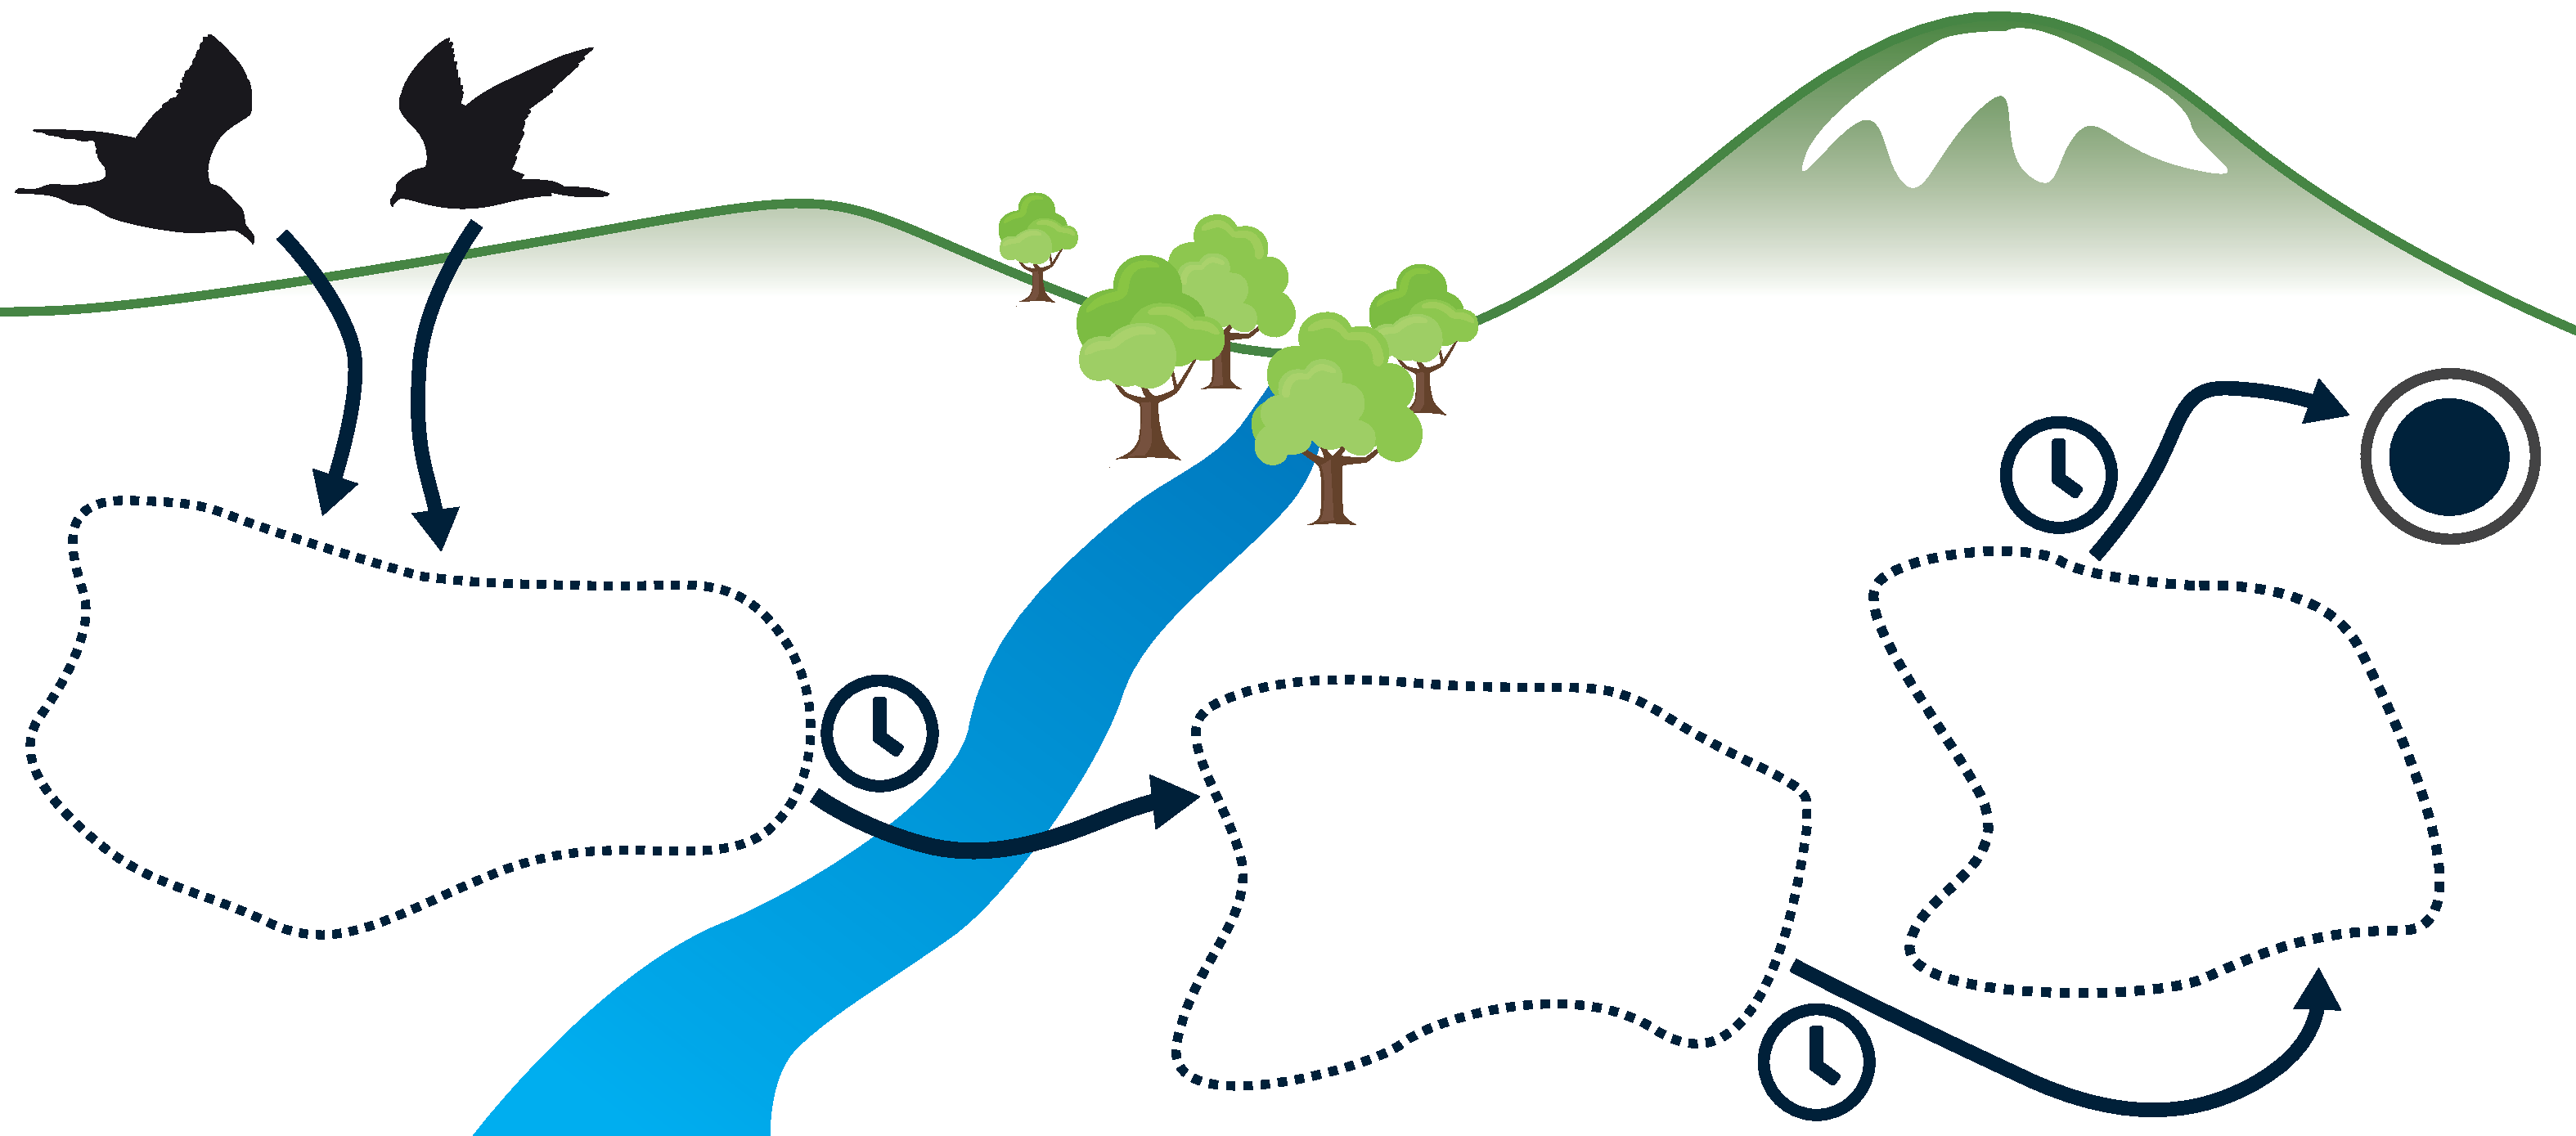
\includegraphics{figures/ch4-gut.pdf}}
    \caption[Give Up Time]{The give up time}
    \label{fig:gut}
\end{figure}

The next two strategies are based on the \emph{time} rule and the \emph{Giving Up} rule~\cite{gibbs1958number_rule}:

\begin{itemize}
    \item[\blueboxbold{SS9}] Employing this stopping strategy, a searcher will leave a SERP after $x_9$ seconds have elapsed from first entering it.
\end{itemize}

\begin{itemize}
    \item[\blueboxbold{SS10}] A searcher employing this strategy will stop after $x_10$ seconds have elapsed since a snippet judged to be relevant was found. If no relevant items have been encountered on the given SERP, then the searcher will stop after $x_9$ seconds have elapsed since arriving at the SERP.
\end{itemize}

These stopping strategies are similar to the frustration based strategies previously proposed (i.e. \textbf{SS2} and \textbf{SS3}) except bound by time~\cite{gibbs1958number_rule}. As mentioned earlier ~\citet{mcnair1982gut_mvt} studied how animals would change their stopping strategies based on their initial evaluation  of the patch, where his suggested combination rule would be as follows.

\begin{itemize}
    \item[\blueboxbold{SS11}] When encountering a SERP expected to yield a high volume of relevant content early on (high scent), the searcher will employ the satisfaction stopping strategy \textbf{SS8S}. If the SERP however yields relevant items over greater depths, or is judged to be of poor quality (low scent), the giving-up stopping strategy, \textbf{SS10G}, is used instead.
\end{itemize}

The combination rule tries to ensure that searcher avoids wasting time on patches with a low yield, but capitalize on patches with a high yield. In the following section, we shall describe the simulated analysis to compare the existing and proposed stopping strategies.

\section{\gls{acr:ir} Evaluation Measures}
As previously mentioned most evaluation measures implicitly encode some stopping model (e.g. P$@$10 encodes SS1$@$10). Two measures that have been recently proposed that explicitly encode a stopping model are \textbf{RBP}~\cite{moffat2008rbp} and \textbf{INST}~\cite{bailey2015inst, moffat2015inst}. 
Under \textbf{RBP}, the decision to continue to the next results is based on the patience parameter (e.g. the probability of continuing), while under \textbf{INST} the probability of continuing is based on how many the documents the searcher expects to encounter, how many they have encountered and their current rank - essentially the probability of continuing decreases as they encounter more relevant information, and as they progress further down the ranking.

\begin{itemize}
    \item[\blueboxbold{SS12}] RBP
\end{itemize}

\begin{itemize}
    \item[\blueboxbold{SS13}] INST
\end{itemize}

The satisfaction stopping strategy \textbf{SS8S} was set to consider $1$ to $7$ (hence providing values for $x_8$). A maximum of seven was chosen as this was closest integer to the mean number of documents marked by subjects in the log data. With our \textbf{INST} stopping strategy employing a similar approach, considering the ``number of useful pages that the searcher expects they will need''~\cite{moffat2015inst}, we subsequently set $T$ in INST to the same range. For our other baseline, \textbf{RBP} considers a \emph{patience factor} that influences the depth to which a searcher is prepared to tolerate examining to. Using the log data we estimated the patience of users to be approximately $p=0.9087$. In this study, examined patience from $0.8$ to $0.95$ in steps of $0.05$, and also $0.99$.